\begin{frame}{Kyber et les anneaux quotients}
    \large{\centerline{\textbf{}}}

\end{frame}

%------------------------------------------------
%------------------------------------------------

\begin{frame}{Kzber \FiveStar \FiveStar\FiveStar \hfill 25 résolutions}
    \begin{columns}[c]
        \column{.45\textwidth}
        \begin{center}                  
            
\includegraphics[width=0.9\textwidth]{img/meme/kyber-intro.png}
        \end{center}

        \column{.65\textwidth} % 
           \begin{outline}
                \1 Objectifs : 
                    \2 Récupérer $\u{k}$ sur 128 bits  chiffré via Kyber
                \1 Données :
                    \2 La clef publique $\k{A}$ et $\k{t}$
                    \2 Le chiffré $E(\u{k})$
                    \2 Le code source
           \end{outline}
    \end{columns}
\end{frame}

%------------------------------------------------
%------------------------------------------------

\begin{frame}{Kyber / ML-KEM (le vrai)}
PQ-KEM (chiffrement asymétrique) standardisé par le NIST
\pause
   \begin{block}{\only<3->{Ring/Module }Learning with Errors (\only<3->{R/M}LwE)}
   Soit $\k{A}\in\mathbb{Z}_q^{k\times k}$.
       \begin{itemize}
        \item Facile de récupérer $\u{s}\in\mathbb{Z}_q^k$ sachant $\k{t}=\k{A}.\u{s}$ (Interpolation)
        \pause
        \item Difficile  de récupérer $\u{s}\in\mathbb{Z}_q^k$ sachant $\k{t}=\k{A}.\u{s}+\u{e}$ où $\u{e}\in\mathbb{Z}_q^{k}$ est petit ($|\u{e}|<\eta$)
        \pause 
        \item Même chose dans $\mathcal{R}_q^k = \left(\mathbb{Z}_q[X]/\left<\phi\right>\right)^k$, et $\phi$ de degré $n$
       \end{itemize}
   \end{block}
   \pause
   \begin{table}
        \begin{tabular}{c|c|c|c|c}
            Nom       & n   & k & q    & $\eta$ \\
            \hline
            Kyber512  & 256 & 2 & 3329 & 2\\
            Kyber768  & 256 & 3 & 3329 & 2\\
            Kyber1024 & 256 & 4 & 3329 & 2\\
        \end{tabular}
    \end{table}
    \pause 
    $\mathcal{R}_q = \mathbb{Z}_q[X]/(X^n+1)$
\end{frame}

\begin{frame}{Algorithmes de Kyber}
    \begin{columns}[c]
        \column{.5\textwidth}
            \begin{outline}
                \1 \textbf{Keygen} : $\k{t} = \k{A}. \u{s}+\u{e}$ 
                    \2 Clef privée $(\u{s})$
                    \2 Clef publique $(\k{A},\k{t})$
                \pause
                \1 \textbf{Chiffrement $m$} : 
                    \2 $\left\{
                \begin{array}{c c l}
                   \k{u} & = & \k{A}^T\u{r} + \u{e_1}\\
                   \k{v} & = & \k{t}^T\u{r}+\u{e_2} + m\\
                \end{array}
                \right.$
                \pause
                \1 \textbf{Déchiffrement $(u,v)$} : 
                    \2 $\k{v}-\u{s}^T\k{u} = m +\u{e}^T\u{r}+\u{e_2} + \u{s}^T\u{e_1} = m + \u{e_3}$
                \end{outline}
        \column{.65\textwidth} % 
        \begin{center}   
            \only<4>{
                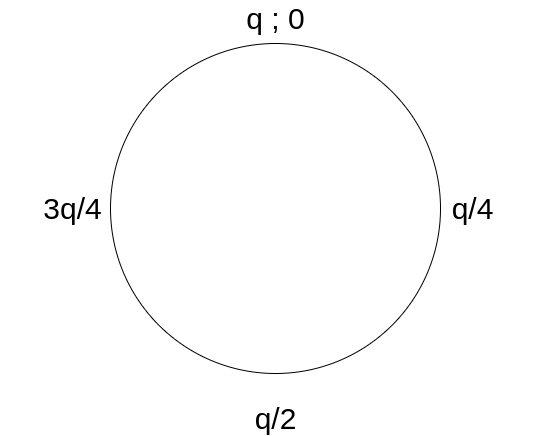
\includegraphics[width=0.8\textwidth]{img/crypto/kyber/kyber-modulo.png}
            }
            \only<5>{
                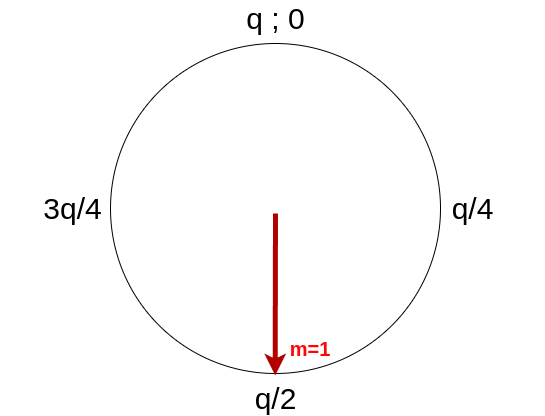
\includegraphics[width=0.8\textwidth]{img/crypto/kyber/kyber-chose_m.png}
            }
            \only<6>{
                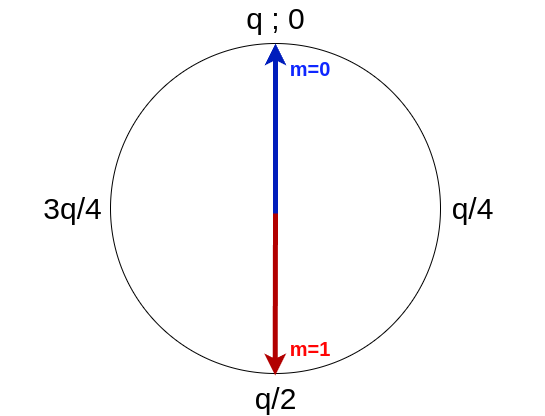
\includegraphics[width=0.8\textwidth]{img/crypto/kyber/kyber-1 or 0.png}
            }
            \only<7>{
                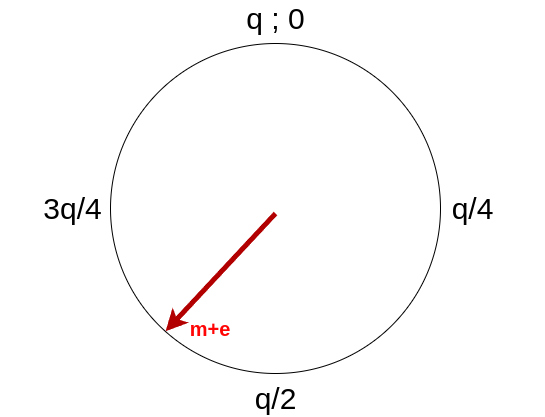
\includegraphics[width=0.8\textwidth]{img/crypto/kyber/kyber-add error.png}
            }
            \only<8->{
                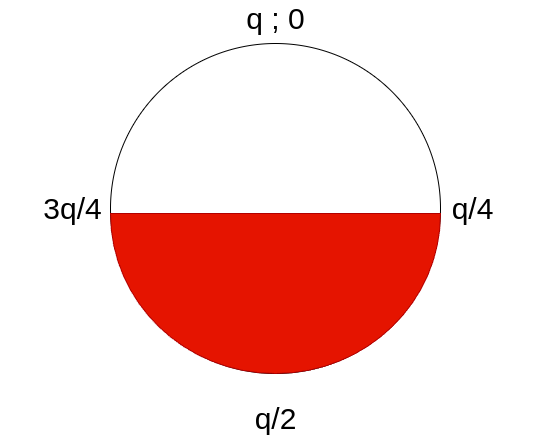
\includegraphics[width=0.8\textwidth]{img/crypto/kyber/kyber-decrypt.png}
            }
        \end{center}
   \end{columns}
   \pause
   $m$ est un polynôme de $\mathcal{R}_q$ (e.g $0101$ devient $0+\frac{q}{2}x+0x^2+\frac{q}{2}x^3$)
\end{frame}

\begin{frame}{Retour au challenge : La (les?) typos}
    \begin{outline}
        \1 $E(m_0),\dots,E(m_k)$ au lieu de $E(m_0,\dots,m_k)$
            \2 $m$ est le polynôme constant 0 ou $q/2$

        \vspace{0.2cm}
        \pause
        
        \1 Travail modulo $X^n\textbf{-}1$ (au lieu de $X^n+1$) qui admet des racines dans $\mathbb{Z}_q$ 
        \pause
            \2 $P\mapsto P(1)$ est un morphisme d'anneau sur $\mathcal{R}_q$ % $\longrightarrow$ somme des coefficients
	    	\3 C'est le morphisme $P \mapsto P \mod X-1$

            \vspace{0.1cm}
            \pause
            
            \2  $\k{v}(1) = \left[\k{t_0}(1),\,\k{t_1}(1)\right]\bullet \left[\u{r_0}(1),\,\u{r_1}(1)\right]^{T}+\u{e_2}(1) + m(1)$ \pause $\in[-q/2,q/2]$ 
            \pause
                \3 $\k{v}(1) = \k{0}+\u{e_2}(1) + m$  avec probabilité $1/q^2$ \hfill ($\sim\frac{1}{11\,082\,241}$)
                \pause
                \3 $\k{v}(1) = \k{\epsilon}\u{r_0}(1)+\k{\epsilon}\u{r_1}(1)+\u{e_2}(1) + m$  avec probabilité $\epsilon^2/q^2$ \hfill ($\sim\frac{1}{12\,313}$)
                \pause
                %\3 Bruteforce des valeurs de $\u{r_0}(1),\u{r_1}(1)$ (à réinjecter dans $\k{v}=\k{A}\cdot\u{r}+\u{e_2}$)

            \vspace{0.1cm}
            \pause
            
            \2 $P\mapsto P(-1)$ est aussi un morphisme d'anneau \hfill ($\sim\frac{1}{6\,156}$)
	    	\3 C'est le morphisme $P \mapsto P \mod X+1$

            \vspace{0.1cm}
            \pause
            
            \2 $X^{256}-1$ à exactement 256 racines dans $\mathbb{Z}_q$ (et $X^{256}+1$ n'en a pas)
		\3 Difficile à exploiter car $\u{e_2}(r)$ est grand
		
		\pause
	    \2 $X^{256}-1$ est divisible par $X^{2^k}-1$  (et $X^{256}+1$ n'en a pas)\hfill ($\sim\frac{1}{96}$)
        \vspace{0.2cm}
        \pause

        \1 On peut générer des instances du problème jusqu'à avoir la solution via au moins l'un de ces morphismes $\flag$

    \end{outline}
\end{frame}
